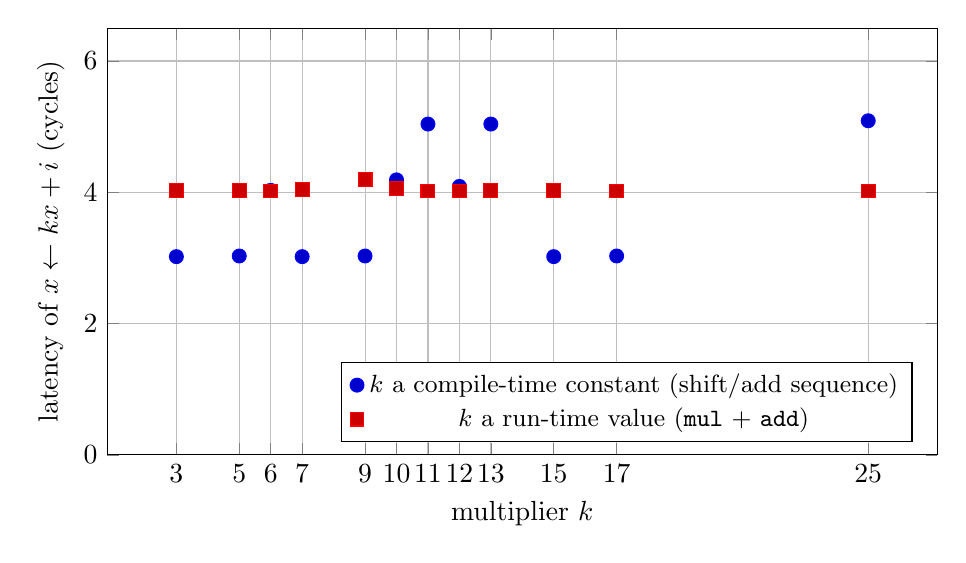
\begin{tikzpicture}
\begin{axis}[width=\textwidth, height=7cm, xlabel={multiplier $k$}, ylabel={latency of $x \leftarrow kx + i$ (cycles)}, grid=major, ymin=0, ymax=6.5,
  xtick={3,5,6,7,9,10,11,12,13,15,17,25}, legend pos=south east, legend style={font=\small}]
\addplot+[only marks, mark=*, mark size=2.5pt, blue] coordinates {(3,3.02) (5,3.03) (6,4.03) (7,3.02) (9,3.03) (10,4.19) (11,5.04) (12,4.09) (13,5.04) (15,3.02) (17,3.03) (25,5.09)};
\addlegendentry{$k$ a compile-time constant (shift/add sequence)}
\addplot+[only marks, mark=square*, mark size=2.5pt, red] coordinates {(3,4.03) (5,4.03) (6,4.02) (7,4.04) (9,4.19) (10,4.06) (11,4.02) (12,4.02) (13,4.03) (15,4.03) (17,4.02) (25,4.02)};
\addlegendentry{$k$ a run-time value (\texttt{mul} + \texttt{add})}
\end{axis}
\end{tikzpicture}